% !TeX root = ../../Book2.tex
% 纲要标题：## 第3章　胞腔同调、映射度与实际计算
% 纲要位置：几何学计划纲要.md，第 1067 行。
% 正文状态：未撰写；本文件目前是框架。

% 纲要内容开始
% 
% > 本章目标与证明范围：完整比较胞腔链与奇异链，使用整数矩阵保留挠信息。将附着映射、映射度和边界矩阵放在同一证明流程中。
% 
% 纲要内容结束

\chapter{胞腔同调、映射度与实际计算}
\label{g2:ch:03}
\BookChapterNumber{g2:ch:03}

\begin{chapterabstract}
待撰写
\end{chapterabstract}

\begin{learninggoals}
待撰写
\end{learninggoals}

待撰写

% !TeX root = ../../Book2.tex
% 纲要标题：### 3.1 骨架滤过给出的链复形
% 纲要位置：几何学计划纲要.md，第 1121 行。
% 正文状态：初稿；尚未正式审核。

% 纲要内容开始
% 
% * 骨架对的相对同调
% * 连接映射与胞腔微分
% * 胞腔微分平方为零
% * 与奇异同调的自然比较
% 
% 纲要内容结束

\section{骨架滤过给出的链复形}
\label{g2:sec:0301}

奇异链复形允许所有连续单形，因而适用于任意空间；但即使空间只有一个点，链群也在每个非负次数都有生成元。第一章给出的胞腔分解则只记录空间实际怎样由圆盘拼成。我们希望每个定向的 \(n\) 胞腔只贡献一个 \(n\) 维生成元，同时保留奇异同调中的全部信息。

\ProseParagraphBreak

困难在于胞腔的边界不必嵌入旧骨架，甚至可能多次经过同一个低维胞腔。因此不能把它简单当成若干几何面的集合。本节先用相对同调把每个圆盘的内部单独取出，再由连接同态恢复其附着边界。全节使用整数系数，约定 \(X^{-1}=\varnothing\)，普通同调在负次数为零。

\subsection{骨架对的相对同调}
\label{g2:subsec:0301:01}
相对同调 \(H_q(X^n,X^{n-1})\) 把旧骨架中的链视为零。每个新圆盘的边界因而消失，留下的应当是一个球面的顶维类。下面的切除论证说明，这个直观在胞腔数无限、附着映射不单射时仍然成立。

\begin{theorem}[骨架对的相对同调]\label{g2:thm:skeletal-relative-homology}
	设 \(X\) 为 CW 复形，\(E_n\) 为其 \(n\) 胞腔的指标集，\(\phi_\alpha:(D^n_\alpha,S^{n-1}_\alpha)\to(X^n,X^{n-1})\) 为特征映射。对所有整数 \(q\ge0\)，这些映射诱导同构
	\[
		\bigoplus_{\alpha\in E_n}H_q(D^n_\alpha,S^{n-1}_\alpha)
		\xrightarrow{\ \cong\ }H_q(X^n,X^{n-1}).
	\]
	当 \(n=0\) 时，将圆盘边界理解为空集。因此右边在 \(q\ne n\) 时为零，在 \(q=n\) 时是以定向 \(n\) 胞腔为基的自由阿贝尔群。同一结论适用于通过附着一族 \(n\) 胞腔得到的空间对 \((Y,A)\)。
\end{theorem}
\begin{proof}
	先处理 \(n\ge1\)。在附着空间 \(Y\) 中，取旧空间 \(A\) 连同各圆盘半径大于 \(1/2\) 的外环所形成的集合 \(U\)。在每个特征圆盘上的原像是 \(\{u:\|u\|>1/2\}\)，在 \(A\) 上的原像是全部 \(A\)，故商拓扑保证 \(U\) 是包含 \(A\) 的开集。外环中的 \(u=r\theta\) 沿
	\[
		r\theta\longmapsto\bigl((1-t)r+t\bigr)\theta
	\]
	推向圆盘边界，并在 \(A\) 上保持不动。这给出 \(U\) 到 \(A\) 的强形变收缩。各圆盘上的公式在边界一致；限制到开集的商映射仍是商映射，而与区间相乘仍为商映射（\cref{g2:lem:quotient-interval}），所以此同伦确实连续。

	由于 \(H_q(U,A)=0\)，三元组序列（\cref{g2:thm:triple-LES}）给出 \(H_q(Y,A)\cong H_q(Y,U)\)。附着构造中 \(A\) 闭，且 \(A\subset U=\operatorname{int}_Y U\)，所以切除定理的闭包条件成立。切去 \(A\) 后，各胞腔内部成为互不相交的开球，得到
	\[
		H_q(Y,U)\cong
		H_q\left(\coprod_{\alpha\in E_n}\mathring D^n_\alpha,
		\coprod_{\alpha\in E_n}\{u:1/2<\|u\|<1\}\right)
		\cong\bigoplus_{\alpha\in E_n}H_q(\mathring D^n,\{1/2<\|u\|<1\}).
	\]
	最后一个同构在链上已经成立：每个奇异单形的参数域连通，像落在一个不交分支中；每条链又只含有限个单形。因此这里是直和，不是允许无限支撑的直积。

	为核对同构恰由特征映射诱导，在每个圆盘中也取外环 \(V=\{u:1/2<\|u\|\le1\}\)。边界是 \(V\) 的强形变收缩核，所以 \(H_q(D^n,S^{n-1})\to H_q(D^n,V)\) 为同构；切除边界又将后者识别为 \(H_q(\mathring D^n,V\setminus S^{n-1})\)。这些映射与 \(\phi_\alpha\) 及前述切除图交换，于是其直和正是陈述中的映射。由\cref{g2:prop:ball-puncture-homology}，每个圆盘对只在次数 \(n\) 贡献一个 \(\mathbb Z\)。

	当 \(n=0\) 时，\(Y\) 是 \(A\) 与新增离散点的不交并，相对链只留下这些点的链复形。单点同调计算直接给出所述结论。取 \(Y=X^n\)、\(A=X^{n-1}\)，即得骨架对的情形。
\end{proof}

这里给胞腔选定向，代数上就是在 \(H_n(D^n,S^{n-1})\cong\mathbb Z\) 中选一个生成元。记它为 \([D^n,S^{n-1}]\)，并把其特征映射下的像记作 \(e^n_\alpha\)。这不会把一个可能自我识别的闭胞腔当成嵌入圆盘；生成元来自参数圆盘的相对同调。

\begin{proposition}[骨架的维数与稳定性]\label{g2:prop:skeletal-homology-stability}
	设 \(X\) 为 CW 复形，\(m,q\ge0\)。则 \(H_q(X^m)=0\) 当 \(q>m\)；包含映射 \(X^m\hookrightarrow X\) 在 \(q<m\) 时诱导同构，在 \(q=m\) 时诱导满射。不要求 \(X\) 有限维或局部有限。
\end{proposition}
\begin{proof}
	在 \((X^r,X^{r-1})\) 的长正合列中考察
	\[
		H_{q+1}(X^r,X^{r-1})\longrightarrow H_q(X^{r-1})
		\longrightarrow H_q(X^r)\longrightarrow H_q(X^r,X^{r-1}).
	\]
	两端只可能分别在 \(r=q+1\)、\(r=q\) 时非零。因此加入 \(r\) 胞腔只可能增加 \(r\) 次同调、消去 \(r-1\) 次同调，其他次数的包含映射均为同构。从离散的 \(X^0\) 开始归纳，便得维数消失性；固定 \(q\)，从 \(X^q\) 到 \(X^{q+1}\) 的映射满射，此后各步均为同构。

	还须说明无限个骨架的并不会出现额外的类或关系。任一奇异链仅含有限个单形，其支撑是紧集，因而由\cref{g2:thm:finite-subcomplex}落在有限子复形中，特别地落在某个有限维骨架中。于是 \(X\) 中的每个 \(q\) 圈可用刚才的有限步结论移到 \(X^q\)；如果 \(X^m\) 中的一个圈在 \(X\) 中成为边界，那么实现这个关系的有限链也落在某个骨架 \(X^r\) 中。当 \(q<m\) 时，\(H_q(X^m)\to H_q(X^r)\) 已是同构，故原圈在 \(X^m\) 中就是边界。这分别给出满射与单射。
\end{proof}

\subsection{连接映射与胞腔微分}
\label{g2:subsec:0301:02}
现在每个维数都有所需的自由群，但各维群之间还没有边界映射。一个 \(n\) 胞腔的边界首先给出 \(X^{n-1}\) 中的绝对同调类；再忽略更低的 \(X^{n-2}\)，才得到 \((n-1)\) 胞腔的线性组合。这两步不能颠倒，也不能把其中的相对化步骤省去。

\begin{definition}[胞腔链复形]\label{g2:def:cellular-chain-complex}
	设 \(X\) 为 CW 复形。定义其整数\term[bao qiang lian qun]{胞腔链群}[cellular chain group]为
	\[
		C_n^{\mathrm{cell}}(X)=H_n(X^n,X^{n-1})\quad(n\ge0),\qquad
		C_n^{\mathrm{cell}}(X)=0\quad(n<0).
	\]
	记空间对的连接同态为 \(\delta_n:H_n(X^n,X^{n-1})\to H_{n-1}(X^{n-1})\)，相对化同态为 \(j_r:H_r(X^r)\to H_r(X^r,X^{r-1})\)。定义\term[bao qiang wei fen]{胞腔微分}[cellular differential]
	\begin{equation}\label{g2:eq:cellular-differential}
		\mathrm{d}_n=j_{n-1}\delta_n:C_n^{\mathrm{cell}}(X)\longrightarrow C_{n-1}^{\mathrm{cell}}(X)\quad(n\ge1),\qquad \mathrm{d}_0=0.
	\end{equation}
	下文证明这些同态组成链复形，称为\term[bao qiang lian fu xing]{胞腔链复形}[cellular chain complex]，其同调记为 \(H_n^{\mathrm{cell}}(X)\)。
\end{definition}

\symidx{\(C_n^{\mathrm{cell}}(X)\)：胞腔链群}
\symidx{\(H_n^{\mathrm{cell}}(X)\)：胞腔同调群}
这一定义中的 \(C_n^{\mathrm{cell}}\) 本身已经是一个相对同调群；在它们之间再取核与像，才得到胞腔同调。相比之下，奇异链群 \(C_n(X)\) 是由全部连续单形生成的自由群。两种“链”处在不同构造层次，不能直接把一个胞腔符号当成某个唯一的奇异单形。

\ProseParagraphBreak

若 \(c\) 是代表某个胞腔链的奇异相对圈，则 \(\partial c\) 落在 \(X^{n-1}\) 中。\cref{g2:thm:pair-LES}约定连接同态为 \([c]\mapsto[\partial c]\)，没有另加负号；再模去 \(X^{n-2}\) 中的链，就得到 \(\mathrm{d}_n[c]\)。三元组 \((X^n,X^{n-1},X^{n-2})\) 的连接同态正是这个复合。

\begin{example}[有向边的边界]\label{g2:exm:cellular-edge-boundary}
	设一条一胞腔由特征路径 \(\phi:[0,1]\to X^1\) 给出，起点与终点分别为顶点 \(v_-\)、\(v_+\)，以参数从 \(0\) 到 \(1\) 为正方向。由\cref{g2:exm:interval-relative-class}，连接同态给出
	\[
		\mathrm{d}_1 e=[v_+]-[v_-].
	\]
	若两端附着到同一个顶点，结果为零，而不是两倍这个顶点。取两个顶点 \(v,w\)，用三条均从 \(v\) 指向 \(w\) 的边 \(a,b,c\) 相连，则
	\[
		\mathrm{d}_1(xa+yb+zc)=(x+y+z)(w-v).
	\]
	所以一维圈群由 \(b-a,c-a\) 自由生成。图没有二维胞腔，这些圈不会成为胞腔边界；它的胞腔同调为 \(H_1^{\mathrm{cell}}\cong\mathbb Z^2\)、\(H_0^{\mathrm{cell}}\cong\mathbb Z\)。下一小节后的比较定理将说明，这也就是奇异同调。
\end{example}

\subsection{胞腔微分平方为零}
\label{g2:subsec:0301:03}
\begin{proposition}[胞腔微分的复合]\label{g2:prop:cellular-d-square}
	对任意 CW 复形 \(X\) 及整数 \(n\)，胞腔微分满足 \(\mathrm{d}_{n-1}\mathrm{d}_n=0\)。若 \(f:X\to Y\) 是胞腔映射，则空间对映射 \((X^n,X^{n-1})\to(Y^n,Y^{n-1})\) 诱导的同态 \(f_n^{\mathrm{cell}}\) 组成链映射。
\end{proposition}
\begin{proof}
	对于 \(n\ge2\)，由定义有
	\[
		\mathrm{d}_{n-1}\mathrm{d}_n
		=j_{n-2}\delta_{n-1}j_{n-1}\delta_n.
	\]
	空间对 \((X^{n-1},X^{n-2})\) 的长正合列中，\(j_{n-1}\) 与 \(\delta_{n-1}\) 是相邻的两条映射，故 \(\delta_{n-1}j_{n-1}=0\)。在代表链上，这也表示绝对圈已经没有边界。\(n\le1\) 时结论由 \(\mathrm{d}_0=0\) 及负次数链群为零得到。

	胞腔映射保持每层骨架；空间对长正合列的自然性给出
	\[
		(f|_{X^{n-1}})_*\delta_n^X=\delta_n^Y f_n^{\mathrm{cell}},\qquad
		f_{n-1}^{\mathrm{cell}}j_{n-1}^X=j_{n-1}^Y(f|_{X^{n-1}})_*.
	\]
	复合两式，便得 \(\mathrm{d}_n^Yf_n^{\mathrm{cell}}=f_{n-1}^{\mathrm{cell}}\mathrm{d}_n^X\)，这就是链映射条件。
\end{proof}

\(\mathrm{d}^2=0\) 因而不是对附着图逐个猜测所得的巧合，而是长正合列的结构保证。实际计算出整数边界矩阵后，矩阵乘积为零仍值得核对：理论保证正确输入满足它，计算中漏掉一次经过或弄反一个方向，却会破坏这个条件。

\ProseParagraphBreak

反转一个胞腔的定向只把相应生成元乘以 \(-1\)。如果在第 \(n\) 维用对角矩阵 \(P_n\) 记录这些符号变化，边界矩阵按 \(A_n\mapsto P_{n-1}^{-1}A_nP_n\) 改变，故新旧链复形同构。胞腔的定向是写矩阵的选择，同调群并不依赖这一选择。

\subsection{与奇异同调的自然比较}
\label{g2:subsec:0301:04}
关键问题现在变成：胞腔圈对应哪些奇异圈，胞腔边界对应哪些奇异边界？先看 \(n\) 骨架上的绝对同调，再只加入下一层胞腔，就足以回答这两个问题。

\begin{theorem}[胞腔同调与奇异同调]\label{g2:thm:cellular-singular-comparison}
	设 \(X\) 为任意 CW 复形，使用整数系数。对每个 \(n\ge0\)，存在同构
	\[
		\Theta_{X,n}:H_n^{\mathrm{cell}}(X)\xrightarrow{\ \cong\ }H_n(X),
	\]
	并且对胞腔映射自然：若 \(f:X\to Y\) 为胞腔映射，则
	\[
		\Theta_{Y,n}H_n(f^{\mathrm{cell}})=f_*\Theta_{X,n}.
	\]
	若给任意连续映射取胞腔逼近，这个公式也确定其在胞腔同调上的同态，且与逼近的选择无关。
\end{theorem}
\begin{proof}
	当 \(n\ge1\) 时，\(H_n(X^{n-1})=H_{n-1}(X^{n-2})=0\)，这里 \(n=1\) 的第二项为 \(H_0(\varnothing)=0\)。两个空间对的长正合列于是说明
	\[
		j_n:H_n(X^n)\hookrightarrow C_n^{\mathrm{cell}}(X),\qquad
		j_{n-1}:H_{n-1}(X^{n-1})\hookrightarrow C_{n-1}^{\mathrm{cell}}(X)
	\]
	都是单射。因 \(\mathrm{d}_n=j_{n-1}\delta_n\)，第二条单射保证 \(\ker\mathrm{d}_n=\ker\delta_n\)；第一条正合列再给出
	\begin{equation}\label{g2:eq:cellular-cycles-skeleton}
		j_n:H_n(X^n)\xrightarrow{\ \cong\ }\ker\mathrm{d}_n.
	\end{equation}
	这表明胞腔圈恰是 \(n\) 骨架上的奇异同调类。并不是每个胞腔链都能提升为绝对圈：能否提升，正由 \(\delta_n\) 检测。

	接着考察加入 \((n+1)\) 胞腔后发生的变化。相对项 \(H_n(X^{n+1},X^n)\) 为零，所以空间对序列给出
	\[
		C_{n+1}^{\mathrm{cell}}(X)\xrightarrow{\delta_{n+1}}H_n(X^n)
		\longrightarrow H_n(X^{n+1})\longrightarrow0.
	\]
	由\cref{g2:prop:skeletal-homology-stability}，\(H_n(X^{n+1})\to H_n(X)\) 是同构。因此
	\[
		H_n(X)\cong H_n(X^n)/\operatorname{im}\delta_{n+1}.
	\]
	在 \(j_n\) 下，分母的像恰为 \(\operatorname{im}(j_n\delta_{n+1})=\operatorname{im}\mathrm{d}_{n+1}\)，分子由 \eqref{g2:eq:cellular-cycles-skeleton} 恰对应 \(\ker\mathrm{d}_n\)。取商即得所需同构。\(n=0\) 时，\(j_0:H_0(X^0)\to H_0(X^0,\varnothing)\) 就是恒等识别，\(\ker\mathrm{d}_0=C_0^{\mathrm{cell}}(X)\)；同一段关于 \((X^1,X^0)\) 的正合列和稳定性证明仍然适用。

	为看清同构的选择无关性，给定胞腔圈 \(z\)，先取由单射 \(j_n\) 唯一确定的类 \(\xi\in H_n(X^n)\)，满足 \(j_n\xi=z\)，再将 \(\xi\) 映入 \(H_n(X)\)。若 \(z\) 改变一个胞腔边界，\(\xi\) 恰改变一个 \(\operatorname{im}\delta_{n+1}\) 中的类，它在 \(X\) 中为零。这就是 \(\Theta_{X,n}\) 的具体构造。

	对胞腔映射，包含、相对化与连接映射全部自然，故刚才的核、像和取商识别与 \(f\) 交换。可将结果画成
	\[
		\begin{tikzcd}[column sep=large,row sep=large]
			H_n^{\mathrm{cell}}(X) \arrow[r,"\Theta_{X,n}","\cong"'] \arrow[d,"H_n(f^{\mathrm{cell}})"']
				& H_n(X) \arrow[d,"f_*"] \\
			H_n^{\mathrm{cell}}(Y) \arrow[r,"\Theta_{Y,n}","\cong"']
				& H_n(Y).
		\end{tikzcd}
	\]
	最后，由\cref{g2:thm:cellular-approximation}，任意连续映射 \(f\) 都有同伦的胞腔代表 \(f'\)。奇异同调的同伦不变性给出 \(f'_*=f_*\)，所以对应的胞腔同态必为 \(\Theta_{Y,n}^{-1}f_*\Theta_{X,n}\)，与 \(f'\) 的选择无关。其恒等与复合性质也由这个公式得到。
\end{proof}

这个比较是同调群上的自然比较。它没有声称每个胞腔天然指定一条唯一的奇异链，也没有声称同伦映射在胞腔链群上总是给出相同矩阵；稳定的是取同调后的映射。不同 CW 分解也通过同一个奇异同调得到同构，这为本章最后的计算核对提供依据。上述构造可与\cite[第2.2节，Cellular Homology]{Hatcher2002}对照。

\begin{theorem}[CW 对的胞腔同调]\label{g2:thm:relative-cellular-comparison}
	设 \(X\) 为 CW 复形，\(A\subset X\) 为子复形。包含诱导胞腔子链复形 \(C_\bullet^{\mathrm{cell}}(A)\subset C_\bullet^{\mathrm{cell}}(X)\)。令
	\[
		C_\bullet^{\mathrm{cell}}(X,A)=C_\bullet^{\mathrm{cell}}(X)/C_\bullet^{\mathrm{cell}}(A).
	\]
	其第 \(n\) 群以 \(X\) 中不属于 \(A\) 的定向 \(n\) 胞腔为基，边界由原边界删除属于 \(A\) 的项得到，并有对胞腔空间对映射自然的同构
	\[
		H_n(C_\bullet^{\mathrm{cell}}(X,A))\cong H_n(X,A;\mathbb Z)\qquad(n\ge0).
	\]
\end{theorem}
\begin{proof}
	包含映射在各相对骨架同调上把一个胞腔生成元映到同名生成元，因此逐次单射；它与胞腔微分交换，故确实给出子链复形。商群的基与边界公式随之成立。

	为把这个商复形与奇异相对同调比较，令 \(F_{-1}=A\)、\(F_r=A\cup X^r\)。\cref{g2:prop:cw-pair-relative}说明 \(F_r\) 由 \(F_{r-1}\) 附着那些不在 \(A\) 中的 \(r\) 胞腔得到，拓扑也与 \(X\) 中的子空间拓扑一致。骨架相对同调定理的附着版本给出
	\[
		H_q(F_r,F_{r-1})=0\quad(q\ne r),\qquad
		H_r(F_r,F_{r-1})\cong C_r^{\mathrm{cell}}(X,A).
	\]
	由三元组 \((F_r,F_{r-1},A)\) 的正合列，从 \(H_q(F_{-1},A)=0\) 开始归纳，得到 \(H_q(F_r,A)=0\) 当 \(q>r\)；固定 \(q\)，包含诱导的群在 \(r\ge q+1\) 后稳定。与绝对情形相同，奇异相对圈及实现其边界关系的链都有紧支撑，所以稳定值正是 \(H_q(X,A)\)。

	用三元组序列替换上一证明中的空间对序列，便有单射
	\[
		H_n(F_n,A)\hookrightarrow H_n(F_n,F_{n-1})=C_n^{\mathrm{cell}}(X,A),
	\]
	其像为相对胞腔圈群；下一层的连接映射给出该单射下的全部相对胞腔边界，并且
	\[
		H_n(X,A)\cong H_n(F_n,A)/\operatorname{im}\bigl(H_{n+1}(F_{n+1},F_n)\to H_n(F_n,A)\bigr).
	\]
	这里的微分与商复形的微分相同，因为两者均由代表链取边界，再忽略 \(A\) 及低一层骨架得到。取商于是给出陈述的同构；自然性仍来自三元组序列的自然性。整个论证在 \(n=0\) 也适用，因为 \(H_0(F_{-1},A)=0\)。
\end{proof}

例如，若 \(Y=X\cup_\alpha D^m\)，其中 \(X\) 为 CW 复形且 \(\alpha:S^{m-1}\to X^{m-1}\)，那么相对胞腔链只有次数 \(m\) 的一个 \(\mathbb Z\)，故 \(H_m(Y,X)=\mathbb Z\)，其余次数为零。这个相对群只记录新增胞腔；它的边界究竟消去旧空间的哪个类，仍须回到连接同态及附着映射去计算。
% 纲要条目排为编号小节标题，并进入目录与书签；说明段仍保留于纲要注释中。

% !TeX root = ../../Book2.tex
% 纲要标题：### 3.2 附着映射和边界系数
% 纲要位置：几何学计划纲要.md，第 1128 行。
% 正文状态：初稿；尚未正式审核。

% 纲要内容开始
% 
% * 球面映射度的同调定义
% * 局部度、复合与悬挂
% * 边界系数的度公式
% * 射影空间附着映射的核验
% 
% 纲要内容结束

\section{附着映射和边界系数}
\label{g2:sec:0302}

上一节把每个定向胞腔变成链群的一名基元，尚须回答：一个 \(n\) 胞腔的边界，在某个 \(n-1\) 胞腔上究竟出现多少次？这里的“多少次”必须带符号；两个覆盖片可能相加，也可能抵消。先研究球面映射对唯一的顶维同调生成元做了什么，再将附着映射压到一颗目标球面，就能逐项读出边界矩阵。

\subsection{球面映射度的同调定义}
\label{g2:subsec:0302:01}

由\cref{g2:thm:sphere-homology}，\(n\ge1\) 时 \(H_n(S^n;\mathbb Z)\cong\mathbb Z\)。选择一个生成元 \([S^n]\) 相当于在同调意义下给球面选定向，另一个选择是 \(-[S^n]\)。任何这个群的自同态都只能是乘一个整数，这正是连续映射可以留下的顶维信息。

\begin{definition}[球面映射度]\label{g2:def:sphere-degree}
	设 \(n\ge1\)，\(f:S^n\rightarrow S^n\) 连续。唯一满足
	\[
		f_*[S^n]=(\deg f)[S^n]
	\]
	的整数称为 \(f\) 的\term[yingshe du]{映射度}[degree]。自映射的源和目标使用同一个生成元，故同时更换生成元的符号不改变 \(\deg f\)。若源、目标是两颗分别定向的 \(n\) 维球面，则以各自的正生成元定义映射度；只反转其中一端的定向会改变映射度的符号。\symidx{\(\deg f\)：定向球面之间的映射度}
\end{definition}

当 \(n=0\) 时，可以在 \(\widetilde H_0(S^0)=\mathbb Z([+]-[-])\) 上作同样定义。恒等映射、交换两点的映射与常值映射的度分别为 \(1,-1,0\)。普通 \(H_0(S^0)\) 的秩是二，不能直接把它的任意自同态称为“乘一个整数”；这里使用约化同调是实质性的区别。

\begin{proposition}[映射度的基本性质]\label{g2:prop:degree-basic}
	设 \(n\ge1\)，\(f,g:S^n\rightarrow S^n\) 连续。恒等映射的度为 \(1\)，同伦的映射具有相同的度，并且
	\[
		\deg(g\circ f)=(\deg g)(\deg f).
	\]
	若 \(f\) 不是满射，则 \(\deg f=0\)；若 \(f\) 是同伦等价，则 \(\deg f\in\{1,-1\}\)。这些结论对用约化零次同调定义的 \(S^0\) 映射度也成立。
\end{proposition}
\begin{proof}
	恒等映射与复合公式直接来自同调的函子性。例如
	\[
		(g\circ f)_*[S^n]=g_*\bigl((\deg f)[S^n]\bigr)
		=(\deg f)(\deg g)[S^n].
	\]
	同伦不变性来自\cref{g2:thm:singular-homotopy-invariance}。若 \(y\notin f(S^n)\)，则 \(f\) 分解经过 \(S^n\setminus\{y\}\)，后者同胚于 \(\mathbb R^n\)，因而可缩，其 \(n\) 次同调为零。故 \(f_*=0\)。若 \(h\) 是 \(f\) 的同伦逆，则 \((\deg h)(\deg f)=\deg(hf)=1\)，两个整数只能同为 \(1\) 或同为 \(-1\)。\(S^0\) 的结论可直接检查三类映射，也可使用相同的约化同调论证。
\end{proof}

特别地，非零映射度强迫满射，而零伦映射的度为零。这两条判断的反向含义不能混为一谈：一个映射可以覆盖整个球面，却让不同部分的同调贡献互相抵消。下面的局部公式将把这种抵消写成真正的整数加法。

\subsection{局部度、复合与悬挂}
\label{g2:subsec:0302:02}

先解决最基本的正负号。将球面上下两个半球交换，赤道上的点保持不动；由于同调类的共同边界在两个半球中以相反符号出现，这个交换应当反转顶维生成元。

\begin{proposition}[反射与对径映射]\label{g2:prop:reflection-antipodal-degree}
	设 \(n\ge0\)。球面 \(S^n\subset\mathbb R^{n+1}\) 关于任一过原点超平面的反射，映射度为 \(-1\)。对径映射 \(A_n(x)=-x\) 的映射度为
	\[
		\deg A_n=(-1)^{n+1}.
	\]
	\(n=0\) 时度取约化零次同调的定义。
\end{proposition}
\begin{proof}
	\(n=0\) 时反射交换两个点，将 \([+]-[-]\) 送到其负元。设 \(n\ge1\)，先取反射 \(r(x_1,\ldots,x_n,t)=(x_1,\ldots,x_n,-t)\)。沿用\cref{g2:thm:sphere-homology}的开覆盖 \(U=S^n\setminus\{S\}\)、\(V=S^n\setminus\{N\}\)，连接同构为
	\[
		\delta:\widetilde H_n(S^n)\xrightarrow{\cong}
		\widetilde H_{n-1}(U\cap V)\cong\widetilde H_{n-1}(S^{n-1}).
	\]
	把代表圈细分后写为 \(z=a+b\)，其中 \(a\) 位于 \(U\)、\(b\) 位于 \(V\)。按\cref{g2:eq:mayer-vietoris-connecting}的约定，\(\delta[z]=[\partial a]\)。反射交换 \(U,V\)，所以 \(r_\#z\) 的 \(U\) 部分是 \(r_\#b\)，从而
	\[
		\delta r_*[z]=[\partial r_\#b]
		=-r_*[\partial a].
	\]
	赤道投影 \(U\cap V\rightarrow S^{n-1}\) 与 \(r\) 复合后不变，因此 \(r\) 在交集的同调上诱导恒等。这就给出 \(\delta r_*=-\delta\)，而 \(\delta\) 是同构，故 \(\deg r=-1\)。任一过原点超平面的反射都是 \(h r h^{-1}\)，其中 \(h\) 为正交线性映射限制在球面上的同胚；复合公式使 \(\deg h\) 与 \(\deg h^{-1}\) 抵消，仍得到 \(-1\)。最后，\(A_n\) 是分别改变 \(n+1\) 个坐标符号的反射之复合，所以其度为 \((-1)^{n+1}\)。
\end{proof}

要把整体的度拆成各原像点的贡献，先把球面的生成元限制到一点附近。对 \(x\in S^n\)、\(n\ge1\)，由于 \(S^n\setminus\{x\}\) 非空可缩，约化对的长正合列给出同构
\[
	H_n(S^n)\xrightarrow{\cong}H_n(S^n,S^n\setminus\{x\}).
\]
记 \([S^n]_x\) 为 \([S^n]\) 的像。\cref{g2:prop:local-homology-neighborhood}又将它识别为任意开邻域对 \((U,U\setminus\{x\})\) 的生成元。这样定义的局部正号来自同一个整体选择，各点之间不必另外任意指定符号。

\begin{definition}[局部度]\label{g2:def:local-degree}
	设 \(n\ge1\)，\(f:S^n\rightarrow S^n\) 连续，\(f(x)=y\)，且 \(x\) 是 \(f^{-1}(y)\) 的孤立点。取开邻域 \(U\ni x\)，使 \(U\cap f^{-1}(y)=\{x\}\)。空间对映射
	\[
		f:(U,U\setminus\{x\})\longrightarrow(S^n,S^n\setminus\{y\})
	\]
	在 \(n\) 次同调上将局部正生成元送到 \(\deg_x(f)\,[S^n]_y\)；整数 \(\deg_x(f)\) 称为 \(f\) 在 \(x\) 处的\term[ju bu du]{局部度}[local degree]。缩小 \(U\) 所诱导的局部同调同构与 \(f_*\) 交换，所以该整数与邻域选择无关。\symidx{\(\deg_x(f)\)：映射在孤立原像点处的局部度}
\end{definition}

局部度的定义只要求连续性和孤立原像，并未要求可微或局部可逆。若 \(f\) 将 \(x\) 的某个邻域同胚地映到 \(y\) 的邻域，局部同调同态是同构，故局部度只能为 \(\pm1\)；这时称局部正生成元被保持或反转，分别就是符号 \(+1\) 与 \(-1\) 的含义。

\begin{theorem}[局部度求和]\label{g2:thm:local-degree-sum}
	设 \(n\ge1\)，\(f:S^n\rightarrow S^n\) 连续。如果某点 \(y\) 的原像是有限集 \(F=\{x_1,\ldots,x_r\}\)，则
	\begin{equation}\label{g2:eq:local-degree-sum}
		\deg f=\sum_{i=1}^r\deg_{x_i}(f).
	\end{equation}
	允许 \(F\) 为空，此时右端为空和 \(0\)。特别地，同胚在每一点的局部度都等于其整体映射度。
\end{theorem}
\begin{proof}
	空原像的情形已经包含在\cref{g2:prop:degree-basic}中。设 \(r>0\)，取两两不交的开邻域 \(U_i\ni x_i\)。记 \(U=\bigcup_iU_i\)。在空间对 \((S^n,S^n\setminus F)\) 中切去闭集 \(S^n\setminus U\)；它包含于开集 \(S^n\setminus F\)，满足\cref{g2:thm:singular-excision}的闭包条件。由切除及不交并的链群分解，得到
	\[
		H_n(S^n,S^n\setminus F)
		\cong\bigoplus_{i=1}^r H_n(U_i,U_i\setminus\{x_i\}).
	\]
	限制到单个点 \(x_i\) 对应于投影到第 \(i\) 项：其余 \(U_j\) 在该相对群中已被全部除去。于是整体生成元 \([S^n]\) 在这个直和中的像正是各局部正生成元组成的向量 \((1,\ldots,1)\)，而不是任意选出的 \(r\) 个符号。

	由空间对映射的自然性，以下方块交换，其中上方箭头包含上述切除同构的逆，右方箭头是各 \(f|_{U_i}\) 所诱导同态之和：
	\[
		\begin{tikzcd}[column sep=large,row sep=large]
			H_n(S^n) \arrow[r] \arrow[d,"f_*"'] & \displaystyle\bigoplus_i H_n(U_i,U_i\setminus\{x_i\}) \arrow[d,"\sum_i(f|_{U_i})_*"] \\
			H_n(S^n) \arrow[r,"\cong"'] & H_n(S^n,S^n\setminus\{y\}).
		\end{tikzcd}
	\]
	沿右边走，\((1,\ldots,1)\) 变成 \(\sum_i\deg_{x_i}(f)\)；沿左边走，生成元变成 \(\deg f\) 倍。因此交换性给出公式。同胚的每个目标点只有一个原像，遂得到最后一项。
\end{proof}

在连续映射中，直接按原像点的个数计数一般会错。局部同胚也可能反转符号；若原像虽孤立但映射并不局部可逆，单点的局部度甚至可以是任意整数。公式中每一项都要由相应的局部同调同态决定。

\begin{proposition}[局部复合与悬挂]\label{g2:prop:degree-composition-suspension}
	设 \(f,g:S^n\rightarrow S^n\) 连续，\(n\ge1\)，\(f(x)=y\)、\(g(y)=z\)。若 \(x\) 是 \(f^{-1}(y)\) 的孤立点，\(y\) 是 \(g^{-1}(z)\) 的孤立点，则 \(x\) 是 \((g\circ f)^{-1}(z)\) 的孤立点，且
	\[
		\deg_x(g\circ f)=\deg_x(f)\deg_y(g).
	\]
	此外，对任意 \(n\ge0\) 的球面映射 \(f:S^n\rightarrow S^n\)，其悬挂 \(Sf:S^{n+1}\rightarrow S^{n+1}\) 满足 \(\deg(Sf)=\deg f\)；\(n=0\) 的右端取约化同调定义。
\end{proposition}
\begin{proof}
	先取开邻域 \(V\ni y\)，使 \(g^{-1}(z)\cap V=\{y\}\)，再缩小 \(U\ni x\)，使 \(f(U)\subset V\) 且 \(f^{-1}(y)\cap U=\{x\}\)。于是 \((gf)^{-1}(z)\cap U=\{x\}\)，并有空间对映射的复合
	\[
		(U,U\setminus\{x\})\xrightarrow{f}
		(V,V\setminus\{y\})\xrightarrow{g}
		(S^n,S^n\setminus\{z\}).
	\]
	局部同调的函子性使两个整数相乘，得到第一式。

	对于悬挂，\cref{g2:thm:suspension-homology}提供自然同构
	\[
		\delta:\widetilde H_{n+1}(SS^n)\xrightarrow{\cong}\widetilde H_n(S^n),
		\qquad \delta(Sf)_*=f_*\delta.
	\]
	通过该节给出的同胚 \(SS^n\cong S^{n+1}\) 识别源、目标，取两个球面上经 \(\delta\) 对应的生成元。交换等式说明两端的自同态乘同一个整数，因此悬挂保持映射度。两个生成元同时反号不改变结论。
\end{proof}

\begin{example}[任意整数的实现]\label{g2:exm:all-integer-degrees}
	把 \(S^1\) 看成复平面内的单位圆。对任意整数 \(k\)，映射 \(p_k(z)=z^k\) 的度为 \(k\)。当 \(k=0\) 时它为常值。设 \(k>0\)，任意 \(y\in S^1\) 有 \(k\) 个原像；在各原像附近的角坐标中，映射是 \(t\mapsto kt\)，因此局部度为 \(+1\)。具体地，旋转可把源点与目标点移到 \(1\)，旋转同伦于恒等，局部度为 \(1\)；而正伸缩 \(t\mapsto kt\) 与恒等之间的同伦 \(t\mapsto((1-s)k+s)t\) 始终把非零点送到非零点，在足够小的坐标区间内给出空间对同伦。因此局部同调同态不变，局部度求和给出 \(k\)。若 \(k<0\)，则 \(p_k\) 是 \(p_{|k|}\) 与反射 \(z\mapsto\bar z\) 的复合，故其度为 \(-|k|\)。对 \(p_k\) 作 \(n-1\) 次悬挂，就在每个 \(n\ge1\) 的维数得到度为 \(k\) 的 \(S^n\) 自映射。
\end{example}

\subsection{边界系数的度公式}
\label{g2:subsec:0302:03}

固定一个 CW 复形 \(X\)，并给各胞腔选定向。记 \(e^n_\alpha\) 同时表示开胞腔及其在 \(C_n^{\mathrm{cell}}(X)=H_n(X^n,X^{n-1})\) 中的正基元，实际含义由所在位置区分。对一个 \(n-1\) 胞腔 \(e^{n-1}_\beta\)，把 \(X^{n-1}\) 中该开胞腔以外的全部点压成一点，得到商映射
\[
	q_\beta:X^{n-1}\longrightarrow
	X^{n-1}/(X^{n-1}\setminus e^{n-1}_\beta)
	\cong D^{n-1}_\beta/\partial D^{n-1}_\beta\cong S^{n-1}_\beta.
\]
这个商只保留所问胞腔的内部，故应当对应于从链群中提取它的系数。即使 \(X\) 有无限多个胞腔，商映射也连续：它在各特征圆盘上分别是通常的圆盘商映射或常值映射，CW 弱拓扑保证这些限制给出连续映射。

\ProseParagraphBreak

给商球面定向以前，还须核对圆盘的相对生成元确实映成球面的生成元。设 \(k\ge1\)，\(q:D^k\to D^k/S^{k-1}=Q\)，\(*\) 为压缩边界所得的点，取圆盘中心 \(x\)，记 \(\bar x=q(x)\)。径向形变收缩说明 \(S^{k-1}\hookrightarrow D^k\setminus\{x\}\) 是同伦等价；比较约化对的长正合列，得到下面左侧竖箭头为同构。\(Q\) 同胚于 \(S^k\)，且 \(Q\setminus\{\bar x\}\) 可缩，所以右侧竖箭头也为同构。
\[
	\begin{tikzcd}[column sep=large,row sep=large]
		H_k(D^k,S^{k-1}) \arrow[r,"q_*"] \arrow[d,"\cong"'] & H_k(Q,*) \arrow[d,"\cong"] \\
		H_k(D^k,D^k\setminus\{x\}) \arrow[r,"q_*"'] & H_k(Q,Q\setminus\{\bar x\}).
	\end{tikzcd}
\]
下侧箭头同样是同构：在 \(x\) 的一个小开邻域上，\(q\) 是同胚，再用\cref{g2:prop:local-homology-neighborhood}即可。方块由空间对映射诱导而交换，因此上侧 \(q_*\) 是同构。这也覆盖 \(k=1\)，其左侧比较使用的是边界两点的约化零次同调。由此，将相对圆盘的正生成元的商像选为 \(H_k(Q,*)\) 的正生成元，再经 \(H_k(Q)\cong H_k(Q,*)\) 给商球面定向。上面的 \(S^{n-1}_\beta\) 就采用由 \(e^{n-1}_\beta\) 这样确定的定向。

\begin{theorem}[胞腔边界的度公式]\label{g2:thm:cellular-boundary-degree}
	设 \(X\) 为 CW 复形，各胞腔已经选定向，\(n\ge2\)。对 \(n\) 胞腔的特征映射 \(\Phi_\alpha:D^n_\alpha\rightarrow X^n\)，记附着映射为 \(a_\alpha=\Phi_\alpha|_{\partial D^n_\alpha}\)，并给 \(\partial D^n_\alpha\) 取由连接同态传来的边界定向。则胞腔微分为
	\begin{equation}\label{g2:eq:cellular-degree-formula}
		\mathrm{d}_n(e^n_\alpha)=\sum_\beta
		\deg(q_\beta\circ a_\alpha)\,e^{n-1}_\beta.
	\end{equation}
	和式只有有限个非零项。对 \(n=1\)，将定向区间的起点、终点像分别记为 \(v_-,v_+\)，则 \(\mathrm{d}_1(e^1_\alpha)=v_+-v_-\)；若两端映到同一顶点，结果为零。
\end{theorem}
\begin{proof}
	取与 \(e^n_\alpha\) 对应的相对球生成元 \(u_\alpha\in H_n(D^n_\alpha,\partial D^n_\alpha)\)，其连接像是边界球面的正生成元 \([\partial D^n_\alpha]\)。\cref{g2:thm:skeletal-relative-homology}将 \((\Phi_\alpha)_*u_\alpha\) 识别为 \(e^n_\alpha\)。连接同态的自然性以及\cref{g2:def:cellular-chain-complex}中的 \(\mathrm{d}_n=j\delta\) 给出
	\[
		\mathrm{d}_n(e^n_\alpha)
		=j\,(a_\alpha)_*[\partial D^n_\alpha]
		\in H_{n-1}(X^{n-1},X^{n-2}).
	\]
	这里 \(j\) 把绝对同调类送到相对同调类，故目前的公式已经说明边界完全由附着映射决定。

	映射 \(q_\beta\) 把 \(X^{n-2}\) 送到基点 \(*\)，因而诱导
	\[
		(q_\beta)_*:H_{n-1}(X^{n-1},X^{n-2})
		\longrightarrow H_{n-1}(S^{n-1}_\beta,*)\cong\mathbb Z.
	\]
	它把 \(e^{n-1}_\beta\) 送到 \(1\)，把其他胞腔基元送到 \(0\)：前者来自该特征圆盘上的边界压缩及我们选定的目标定向，后者来自常值映射。因此它正是第 \(\beta\) 个坐标投影。在上式两边作用这个投影，所得整数就是 \(q_\beta a_\alpha\) 在球面顶维同调上乘的整数，即其度。由于 \(n-1\ge1\)，这里 \(H_{n-1}(S^{n-1}_\beta)\rightarrow H_{n-1}(S^{n-1}_\beta,*)\) 是同构，不会引入额外的零次分支项。

	附着球面的像是紧集；由\cref{g2:thm:finite-subcomplex}，它包含在有限子复形内。不在该子复形中的 \(e^{n-1}_\beta\) 对应常值复合 \(q_\beta a_\alpha\)，故其系数为零。最后，\(n=1\) 时相对区间生成元可由正向道路代表，连接同态直接给出终点减起点；这正是所述公式，无须将任意顶点集误当作一个零维球面。
\end{proof}

度公式中的符号来自两项选择：源胞腔的定向规定附着球面的边界定向，目标胞腔的定向规定压缩球面的正生成元。反转源胞腔会改变这列边界系数的全部符号，反转目标胞腔则改变对应行的全部符号。链群基随之改变，同调群不变；计算中应保存这些基选择，不能在某个矩阵中单独改一个看起来不顺眼的负号。

\begin{proposition}[附着字的指数和]\label{g2:prop:word-boundary-degrees}
	设 \(X\) 有一个零胞腔、有限个定向一胞腔 \(a_1,\ldots,a_r\)，且某个二胞腔 \(e\) 的附着映射沿有限字 \(w\) 依次遍历这些圆周，字母 \(a_i^{-1}\) 表示反向遍历。若 \(\nu_i(w)\) 为 \(a_i\) 的出现次数减去 \(a_i^{-1}\) 的出现次数，则
	\[
		\mathrm{d}_2(e)=\sum_{i=1}^r\nu_i(w)a_i.
	\]
	只要一般附着映射与上述逐段遍历的映射同伦，同一公式仍成立。
\end{proposition}
\begin{proof}
	压掉除 \(a_i\) 以外的圆周，在剩余开边内部选一点 \(y\)。复合 \(q_i a\) 的原像每出现一个 \(a_i\) 或 \(a_i^{-1}\) 就有一点，其他字母的线段全部落在基点，不贡献原像。正向遍历的局部角坐标是正伸缩，局部度为 \(+1\)；反向遍历再复合一次反射，局部度为 \(-1\)。由局部度求和，复合的度就是 \(\nu_i(w)\)，再代入胞腔边界公式即可。同伦的附着映射经 \(q_i\) 复合后仍同伦，故各映射度不变。
\end{proof}

例如，一个二胞腔沿 \(aba^{-1}b^{-1}\) 附着时，两项指数和都是零，所以它的胞腔边界为零；沿 \(a^2b^2\) 附着时则得到 \(2a+2b\)。两幅粘合图都可能把同一条边用两次，区别在于两次所带的方向。这正是只数边数不能替代边界矩阵的原因。

\subsection{射影空间附着映射的核验}
\label{g2:subsec:0302:04}

\cref{g2:exm:projective-cw}给出了实射影空间每维一个胞腔的模型：在 \(\mathbb RP^n\) 中新添一个 \(n\) 胞腔，其附着映射是
\[
	\pi:S^{n-1}\longrightarrow\mathbb RP^{n-1},\qquad x\longmapsto[x].
\]
这确实是二重覆盖，但边界系数不能据此立刻写成 \(2\)：度公式要求先把低骨架 \(\mathbb RP^{n-2}\) 压掉，并比较两个覆盖片的符号。对径映射的奇偶性正是在这一步进入。

\begin{proposition}[实射影空间的胞腔微分]\label{g2:prop:rp-cellular-boundary}
	对 \(\mathbb RP^N\) 的标准 CW 结构，可以逐维选择胞腔正生成元 \(e^0,\ldots,e^N\)，使每个 \(1\le n\le N\) 满足
	\begin{equation}\label{g2:eq:rp-cellular-boundary}
		\mathrm{d}_n(e^n)=\bigl(1+(-1)^n\bigr)e^{n-1}
		=\begin{cases}2e^{n-1},&n\text{ 为偶数},\\0,&n\text{ 为奇数}.\end{cases}
	\end{equation}
	有限维数 \(N\) 的取值不影响已经选定的低维胞腔和微分。
\end{proposition}
\begin{proof}
	\(n=1\) 时两个端点都附着到唯一的零胞腔，故 \(\mathrm{d}_1=0\)。现在设 \(n\ge2\)，记
	\[
		F_n:S^{n-1}\xrightarrow{\pi}\mathbb RP^{n-1}
		\xrightarrow{q}\mathbb RP^{n-1}/\mathbb RP^{n-2}\cong S^{n-1}.
	\]
	源球面中的赤道 \(x_n=0\) 映入 \(\mathbb RP^{n-2}\)，两个开半球 \(x_n>0\) 与 \(x_n<0\) 则分别同胚地映到目标球面除基点以外的部分。因为每条不在低维射影子空间中的直线恰有两个单位代表，这两个半球上的映射没有其他原像片。

	从已选定的 \(e^{n-1}\) 出发，在北半球取一点 \(x\)。因为 \(F_n\) 在 \(x\) 附近是局部同胚，其局部度为 \(\pm1\)；选择 \(e^n\) 的定向，使这个局部度为 \(+1\)。反转 \(e^n\) 的定向即反转其边界定向，所以总能做到。此时 \(F_n^{-1}(F_n(x))=\{x,-x\}\)。对径映射 \(A_{n-1}\) 满足 \(F_nA_{n-1}=F_n\)，局部复合公式给出
	\[
		\deg_{-x}(F_n)
		=\deg_{-x}(F_nA_{n-1})
		=\deg_x(F_n)\deg_{-x}(A_{n-1})
		=(-1)^n.
	\]
	最后一步使用：对径映射是同胚，其局部度等于整体度，而\cref{g2:prop:reflection-antipodal-degree}在维数 \(n-1\) 给出的符号是 \((-1)^n\)。因此局部度求和给出 \(\deg F_n=1+(-1)^n\)，胞腔边界的度公式便得到结论。按维数递增作定向选择，不会改变此前已经选定的低维生成元，故所有等式可以同时成立。
\end{proof}

\(\mathbb RP^2\) 的附着圆周有两片同向贡献，所以 \(\mathrm{d}_2=2\)；\(\mathbb RP^3\) 新添胞腔的边界球面上两片贡献反向，所以 \(\mathrm{d}_3=0\)。“覆盖了两次”在相邻维数给出了完全不同的整数边界。下一节将把这些整数代回链复形，直接看见 \(\mathbb Z/2\) 挠项从何而来。映射度、局部度和胞腔边界公式的相关论述可参阅\cite[第2.2节，Degree 与 Cellular Homology]{Hatcher2002}。
% 纲要条目排为编号小节标题，并进入目录与书签；说明段仍保留于纲要注释中。

% !TeX root = ../../Book2.tex
% 纲要标题：### 3.3 典型空间的整数同调
% 纲要位置：几何学计划纲要.md，第 1135 行。
% 正文状态：初稿；尚未正式审核。

% 纲要内容开始
% 
% * 实射影空间和复射影空间
% * 可定向及不可定向曲面
% * 透镜空间与扭项
% * 附着一个高维胞腔改变什么
% 
% 纲要内容结束

\section{典型空间的整数同调}
\label{g2:sec:0303}

胞腔链群告诉我们各维有多少个待检查的生成元，附着映射才决定哪些生成元成为圈、哪些圈又成为边界。下面的空间都有很少的胞腔，却已经展示了三种不同现象：边界为零时保留自由生成元，非零整数倍的边界产生有限阶同调类，而新增胞腔也可能使原有关系之间出现新的关系。本节的同调均取整数系数。

\subsection{实射影空间和复射影空间}
\label{g2:subsec:0303:01}

\cref{g2:exm:projective-cw}给出的标准分解中，\(\mathbb RP^N\) 在实维数 \(0,1,\ldots,N\) 各有一个胞腔，\(\mathbb CP^N\) 只在实维数 \(0,2,\ldots,2N\) 各有一个胞腔。两个空间都可以用“逐次加入一条新的坐标轴”构造，但它们相邻维数的链群很不相同：实情形允许非零边界，复情形的每一个边界映射都面对一个零群。

\begin{proposition}[射影空间的同调]\label{g2:prop:projective-integer-homology}
	对整数 \(N\geq1\)，实射影空间的整数同调为
	\[
		H_k(\mathbb RP^N)\cong
		\begin{cases}
			\mathbb Z,&k=0,\text{ 或 }k=N\text{ 且 }N\text{ 为奇数},\\
			\mathbb Z/2,&0<k<N\text{ 且 }k\text{ 为奇数},\\
			0,&\text{其余情形}.
		\end{cases}
	\]
	对整数 \(N\geq0\)，复射影空间的整数同调为
	\[
		H_k(\mathbb CP^N)\cong
		\begin{cases}
			\mathbb Z,&k=0,2,\ldots,2N,\\
			0,&\text{其余情形}.
		\end{cases}
	\]
	\(\mathbb RP^0\) 是单点，只有零次同调为 \(\mathbb Z\)。
\end{proposition}
\begin{proof}
	选用\eqref{g2:eq:rp-cellular-boundary}的相容胞腔定向，实射影空间的链复形在 \(0\) 至 \(N\) 次各为 \(\mathbb Z\)，并且
	\[
		\mathrm{d}_k=
		\begin{cases}
			2,&k\text{ 为正偶数},\\
			0,&k\text{ 为奇数}.
		\end{cases}
	\]
	若 \(0<k<N\) 为奇数，所有 \(k\) 链都是圈，而边界是它们的偶数倍，所以 \(H_k=\mathbb Z/2\)；若 \(k>0\) 为偶数，\(\mathrm{d}_k\) 单射，故该次同调为零。最高次须单独看：没有来自 \(N+1\) 次的边界，所以当 \(N\) 为奇数时 \(H_N=\ker\mathrm{d}_N=\mathbb Z\)，不是 \(\mathbb Z/2\)。零次的唯一生成元也没有非零边界。

	在复情形，奇数次链群为零，因此所有胞腔边界均为零，每个偶数次胞腔都给出一个无限阶同调生成元。两种计算通过\cref{g2:thm:cellular-singular-comparison}与奇异同调一致。
\end{proof}

例如，\(\mathbb RP^2\) 的一胞腔本身不是二维胞腔的边界，但它的两倍是边界。这就是 \(\mathbb Z/2\) 所记录的几何事实。对于阿贝尔群 \(G\)，满足 \(ng=0\) 的非零元素 \(g\)（其中 \(n\) 为某个正整数）称为\term[naoyuan]{挠元}[torsion element]；零元与全部挠元组成\term[naoziqun]{挠子群}[torsion subgroup]。本节标题中的“扭项”指这种有限阶信息，它由整数边界系数 \(2\) 保留下来。

\ProseParagraphBreak

无限射影空间要连同拓扑一起说明。令
\[
	\mathbb RP^\infty=\bigcup_{N\geq0}\mathbb RP^N,
	\qquad
	\mathbb CP^\infty=\bigcup_{N\geq0}\mathbb CP^N,
\]
其中包含映射在齐次坐标末尾补零，并赋予上述胞腔分解的弱拓扑。它们的每条胞腔链仍是有限和。由胞腔比较定理，直接使用无限链复形便得到
\[
	H_k(\mathbb RP^\infty)\cong
	\begin{cases}
		\mathbb Z,&k=0,\\
		\mathbb Z/2,&k>0\text{ 为奇数},\\
		0,&k>0\text{ 为偶数},
	\end{cases}
	\qquad
	H_k(\mathbb CP^\infty)\cong
	\begin{cases}
		\mathbb Z,&k\geq0\text{ 为偶数},\\
		0,&k\geq0\text{ 为奇数}.
	\end{cases}
\]
这里没有最高维胞腔，因而没有实射影奇数维顶部的那个例外。若从有限空间理解同一个计算，\cref{g2:thm:finite-subcomplex}保证每条奇异链的紧像落在某个有限子复形中；一个圈成为边界时，其填充链也只用有限多个胞腔。固定次数的结果因此由足够高的有限阶段决定。

\subsection{可定向及不可定向曲面}
\label{g2:subsec:0303:02}

我们使用两类熟悉的闭曲面模型。\(\Sigma_g\) 表示 \(g\) 个环面的连通和，\(g\geq1\)，并令 \(\Sigma_0=S^2\)；\(N_h\) 表示 \(h\) 个实射影平面的连通和，\(h\geq1\)。连通和是从两个曲面各删去一个开圆盘，再将留下的边界圆周粘合。前一类可定向，后一类不可定向；下面的计算只需它们的具体多边形模型。

\ProseParagraphBreak

环面由正方形按边界词 \(aba^{-1}b^{-1}\) 粘合，\(\mathbb RP^2\) 则由圆盘边界的两段按同向的 \(aa\) 粘合。对两个这样的多边形模型作连通和，可以在各自二维胞腔中挖去小圆盘，再切开一条连接内外边界的弧；粘合后，这两条切缝合成一条可重新合起的边，剩余外边界依次读出原来的两个词。因此逐次连通和给出一个顶点、若干条边和一个二维胞腔，其附着词分别为
\begin{equation}\label{g2:eq:surface-attaching-words}
	\Sigma_g:\quad\prod_{i=1}^g a_i b_i a_i^{-1}b_i^{-1},
	\qquad
	N_h:\quad a_1^2a_2^2\cdots a_h^2.
\end{equation}
在这些模型中，每条多边形边都成对粘合；边的内点有圆盘邻域，顶点周围的小扇形也首尾接成一个圆盘。因而商确为无边界曲面。可定向模型的成对边在多边形边界上反向出现，使二维胞腔的定向在粘合处相容；\(a_i^2\) 则在相应闭路周围反转局部定向。

\begin{proposition}[闭曲面模型的同调]\label{g2:prop:surface-integer-homology}
	设 \(\Sigma_g\) 为 \(g\ge0\) 个柄的闭可定向曲面模型（\(\Sigma_0=S^2\)），\(N_h\) 为 \(h\ge1\) 个实射影平面的连通和，取 \eqref{g2:eq:surface-attaching-words} 的胞腔分解。它们的整数同调由下表给出，所有高于二次的同调均为零。
	\begin{center}
		\begin{tabular}{cccc}
			\toprule
			空间 & \(H_0\) & \(H_1\) & \(H_2\)\\
			\midrule
			\(\Sigma_g\)（\(g\geq0\)） & \(\mathbb Z\) & \(\mathbb Z^{2g}\) & \(\mathbb Z\)\\
			\(N_h\)（\(h\geq1\)） & \(\mathbb Z\) & \(\mathbb Z^{h-1}\oplus\mathbb Z/2\) & \(0\)\\
			\bottomrule
		\end{tabular}
	\end{center}
\end{proposition}
\begin{proof}
	先设 \(g\geq1\)。每条边的两端都是唯一的顶点，所以 \(\mathrm{d}_1=0\)。\cref{g2:prop:word-boundary-degrees}把二维胞腔的边界系数化为附着词中各字母的指数和。在 \(\Sigma_g\) 的词中，每个 \(a_i,b_i\) 都以正负指数各出现一次，故 \(\mathrm{d}_2=0\)。其链复形为
	\[
		0\longrightarrow\mathbb Z\xrightarrow{0}\mathbb Z^{2g}
		\xrightarrow{0}\mathbb Z\longrightarrow0,
	\]
	于是得到第一行。\(g=0\) 时用球面的一零胞腔、一二胞腔分解，结论相同。

	在 \(N_h\) 中，每个字母的指数和是 \(2\)，所以
	\[
		\mathrm{d}_2(1)=2(a_1+\cdots+a_h),\qquad\mathrm{d}_1=0.
	\]
	这个 \(\mathrm{d}_2:\mathbb Z\to\mathbb Z^h\) 单射，故 \(H_2=0\)。令 \(v=a_1+\cdots+a_h\)，则 \(v,a_2,\ldots,a_h\) 是 \(\mathbb Z^h\) 的一组整数基，因为 \(a_1=v-a_2-\cdots-a_h\)。在这组基下只剩一个关系 \(2v=0\)，因此
	\[
		H_1(N_h)=\mathbb Z^h/\langle2v\rangle
		\cong\mathbb Z/2\oplus\mathbb Z^{h-1}.
	\]
	两种模型的一维骨架都连通，零次同调为 \(\mathbb Z\)，没有更高维胞腔。
\end{proof}

这里可以看见“边界抵消”与曲面定向的关系。对 \(\Sigma_g\)，二维胞腔的各对边在整数链中互相抵消，整个胞腔成为一个二维圈。对 \(N_h\)，同向出现的边留下系数 \(2\)，不能得到非零二维圈。这些模型中的顶维圈由此直接从多边形边界的符号算出。

\subsection{透镜空间与扭项}
\label{g2:subsec:0303:03}

实射影三维空间的 \(\mathbb Z/2\) 可以推广成任意 \(\mathbb Z/p\)。设 \(p\geq2\)，\(q\in\mathbb Z\) 与 \(p\) 互素，并记 \(\zeta=e^{2\pi\mathrm{i}/p}\)。在
\[
	S^3=\{(z_1,z_2)\in\mathbb C^2:|z_1|^2+|z_2|^2=1\}
\]
上考虑周期变换
\[
	\rho(z_1,z_2)=(\zeta z_1,\zeta^q z_2).
\]
定义三维\term[toujingkongjian]{透镜空间}[lens space]为
\[
	L(p,q)\coloneqq S^3/\langle\rho\rangle.
\]
\symidx{\(L(p,q)\)：三维透镜空间}这里固定的是商作用的参数约定；有些文献改用透镜面上的旋转角作第二参数，得到的公式会出现 \(q\) 的模 \(p\) 逆元。若 \(\rho^j\) 固定一个点，则至少一个坐标非零；由 \(p\mid j\) 或 \(p\mid qj\) 及互素条件，都得到 \(p\mid j\)。因此该作用自由。有限多个不同像可以用互不相交的小邻域分开，所以商投影是 \(p\) 叶覆盖，商空间是闭三维流形。

\begin{figure}[tbp]
	\centering
	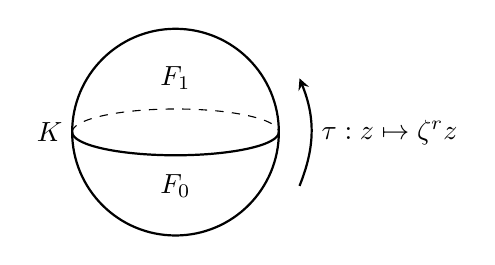
\begin{tikzpicture}[scale=1.05,>=stealth]
		\draw[thick] (0,0) circle (1.25);
		\draw[dashed] (-1.25,0) arc[start angle=180,end angle=0,x radius=1.25,y radius=.28];
		\draw[thick] (-1.25,0) arc[start angle=180,end angle=360,x radius=1.25,y radius=.28];
		\node at (0,.65) {\(F_1\)};
		\node at (0,-.65) {\(F_0\)};
		\node[left] at (-1.25,0) {\(K\)};
		\draw[->,thick] (1.5,-.65) to[bend right=22] node[right] {\(\tau:z\mapsto\zeta^r z\)} (1.5,.65);
	\end{tikzpicture}
	\caption{基本区域三球 \(B\) 的边界示意。两张盘面 \(F_0,F_1\) 沿圆周 \(K\) 相接，并由 \(\tau\) 识别；\(K\) 本身还按 \(p\) 重旋转识别。盘面继承的边界定向相反，边缘的多重绕行则保留在二维边界中。}
	\label{g2:fig:lens-boundary-faces}
\end{figure}

\begin{proposition}[透镜空间的胞腔模型]\label{g2:prop:lens-cellular-model}
	设 \(p\geq2\) 且 \(\gcd(p,q)=1\)。按上述约定定义的 \(L(p,q)\) 有一个在维数 \(0,1,2,3\) 各含一个胞腔的 CW 分解。可以选取胞腔定向，使其整数链复形为
	\begin{equation}\label{g2:eq:lens-cellular-complex}
		0\longrightarrow\mathbb Z\xrightarrow{0}\mathbb Z
		\xrightarrow{p}\mathbb Z\xrightarrow{0}\mathbb Z
		\longrightarrow0.
	\end{equation}
\end{proposition}
\begin{proof}
	我们先找一个基本区域，再读出它的面和边的粘合，\cref{g2:fig:lens-boundary-faces}显示其边界两张盘面的关系。取整数 \(r\) 使 \(rq\equiv1\pmod p\)，并令 \(\tau=\rho^r\)。它仍生成同一个周期群，但在第二坐标上恰旋转 \(2\pi/p\)。在 \(S^3\) 中取扇区
	\[
		B=\left\{\left(z,\sqrt{1-|z|^2}\,e^{\mathrm{i}\theta}\right):
		|z|\leq1,\ 0\leq\theta\leq2\pi/p\right\}.
	\]
	当 \(|z|=1\) 时，第二坐标为零，所有 \(\theta\) 给出同一点。这个集合是闭三球，而不是边界带棱的环面。一个明确的参数说明如下：从普通闭三球 \(\{(z,s):|z|^2+s^2\leq1\}\subset\mathbb C\times\mathbb R\) 出发，在 \(|z|<1\) 时令
	\[
		\theta=\frac{\pi}{p}\left(1+\frac{s}{\sqrt{1-|z|^2}}\right),
	\]
	再代入 \(B\) 的公式；在 \(|z|=1\) 时取 \((z,0)\)。因为趋近边缘时第二坐标的模趋于零，该映射连续；它是紧空间到 Hausdorff 空间的连续双射，故是同胚。

	三球边界分成两个闭圆盘
	\[
		F_j=\left\{\left(z,\sqrt{1-|z|^2}\,e^{2\pi\mathrm{i}j/p}\right):|z|\leq1\right\},
		\qquad j=0,1,
	\]
	它们沿公共圆周 \(K=\{(z,0):|z|=1\}\) 相交。\(\tau\) 把 \(F_0\) 送到 \(F_1\)，在盘坐标中是旋转 \(z\mapsto\zeta^r z\)。若 \(z_2\ne0\) 且其辐角不是 \(2\pi/p\) 的整数倍，该轨道在扇区内部恰有一个代表；若辐角为 \(2\pi/p\) 的整数倍，则在两个盘面内部各有一个代表，它们由上述面粘合识别。剩下的点都位于 \(K\)，其识别为 \(z\sim\zeta z\)。因此从 \(B\) 出发作这些识别，恰得到 \(L(p,q)\)。

	边缘商 \(K/\langle\zeta\rangle\) 是圆周，商坐标可取 \(z\mapsto z^p\)，给它选一个顶点和一条开边。盘面内部的公共像是一开二胞腔，\(B\) 的内部是一开三胞腔；其余点都在刚才的圆周内。这给出所述四个胞腔。它们的特征映射来自圆盘和三球到商空间的映射；空间紧且只有有限多个胞腔，因此附着拓扑与所得商拓扑一致。

	给二胞腔选取 \(F_0\) 的复平面定向，其边界绕 \(K\) 一周；在商圆周中则由 \(z\mapsto z^p\) 绕行 \(p\) 周。因此\cref{g2:thm:cellular-boundary-degree}给出 \(\mathrm{d}_2=p\)。唯一一胞腔的两端相同，故 \(\mathrm{d}_1=0\)。

	最后计算 \(\mathrm{d}_3\)。把三球边界的两个半球都用同一个盘坐标 \(z\) 表示时，它们从三球继承的边界定向相反。两面的识别 \(z\mapsto\zeta^r z\) 又保持盘定向。在二胞腔内部取一点，它在这两个面中各有一个原像，局部度一正一负；压掉一维骨架以后，其度之和为 \(1-1=0\)。这就是 \(\mathrm{d}_3=0\) 的来源。
\end{proof}

两个盘面的定向抵消只说明三胞腔的边界系数为零；二胞腔边缘上的 \(p\) 重绕行仍然存在。由\eqref{g2:eq:lens-cellular-complex}立即得到
\begin{equation}\label{g2:eq:lens-integer-homology}
	H_k(L(p,q))\cong
	\begin{cases}
		\mathbb Z,&k=0,3,\\
		\mathbb Z/p,&k=1,\\
		0,&\text{其余情形}.
	\end{cases}
\end{equation}
一胞腔给出的圈有阶恰为 \(p\)：它的 \(p\) 倍被二胞腔填充，任何较小正倍数都不在 \(p\mathbb Z\) 内。这一计算保留了覆盖重数 \(p\)，却没有保留盘面旋转中的全部参数 \(q\)；因此相同的这组同调群本身不能回答两个透镜空间是否同胚。特别地，\(L(2,1)=\mathbb RP^3\)，与前面的结果吻合。上述胞腔模型也可对照\cite[第2.2节，Cellular Homology]{Hatcher2002}。

\subsection{附着一个高维胞腔改变什么}
\label{g2:subsec:0303:04}

附着球面在旧空间中的同调类，可以是无限阶、有限阶或零。空间对的长正合列分别给出这三种情形中新生成的类与新施加的关系，并说明一次附着只可能影响两个相邻次数的同调。

\begin{proposition}[单胞腔附着的同调变化]\label{g2:prop:single-cell-homology-change}
	设 \(X\) 是非空 CW 复形，\(m\geq2\)，\(\alpha:S^{m-1}\to X^{m-1}\) 连续，并令 \(Y=X\cup_\alpha D^m\)。给圆盘选定向，球面取相应边界定向，记 \(u=\alpha_*[S^{m-1}]\in H_{m-1}(X)\)。则包含 \(X\hookrightarrow Y\) 在 \(k\notin\{m,m-1\}\) 时诱导同构 \(H_k(X)\cong H_k(Y)\)，且有正合列
	\begin{equation}\label{g2:eq:single-cell-six-term}
		\begin{gathered}
			0\longrightarrow H_m(X)\longrightarrow H_m(Y)\longrightarrow\mathbb Z\\
			\xrightarrow{\,1\mapsto u\,}H_{m-1}(X)\longrightarrow H_{m-1}(Y)\longrightarrow0.
		\end{gathered}
	\end{equation}
	特别地，\(H_{m-1}(Y)\cong H_{m-1}(X)/\langle u\rangle\)。若 \(u\) 为无限阶，则 \(H_m(Y)\cong H_m(X)\)；若 \(u\) 有有限阶（包括 \(u=0\)），则存在群同构 \(H_m(Y)\cong H_m(X)\oplus\mathbb Z\)，但后一分解一般没有指定的自然选择。
\end{proposition}
\begin{proof}
	相对胞腔复形 \(C^{\mathrm{cell}}_\bullet(Y,X)\) 只剩新增的一个 \(m\) 次生成元，所有微分为零。由\cref{g2:thm:relative-cellular-comparison}，相对奇异同调为
	\[
		H_k(Y,X)\cong
		\begin{cases}
			\mathbb Z,&k=m,\\
			0,&k\ne m.
		\end{cases}
	\]
	代入\cref{g2:thm:pair-LES}便得到不受影响的次数和\eqref{g2:eq:single-cell-six-term}。还要认清其中的连接同态：特征映射是空间对映射 \((D^m,S^{m-1})\to(Y,X)\)，其相对定向类给出上面 \(\mathbb Z\) 的生成元。连接同态的自然性，以及“取代表链的边界”这一约定，说明它的像恰为 \(\alpha_*[S^{m-1}]=u\)。

	由正合性，低一次群是所述商群，而最高一段可以写成
	\[
		0\longrightarrow H_m(X)\longrightarrow H_m(Y)
		\longrightarrow K\longrightarrow0,
		\qquad K=\{a\in\mathbb Z:au=0\}.
	\]
	若 \(u\) 为无限阶，则 \(K=0\)。若 \(u\) 的阶为 \(s<\infty\)，约定零元的阶为 \(1\)，则 \(K=s\mathbb Z\cong\mathbb Z\)。在 \(H_m(Y)\) 中选一个映到 \(s\) 的元素，它的整数倍给出该短正合列的分裂，因而得到直和分解。更换这个提升可以加上 \(H_m(X)\) 中的元素，所以分解不由原数据唯一指定。
\end{proof}

若 \(u\ne0\) 的阶为 \(s\)，新增胞腔本身的边界还没有消失，但它的 \(s\) 倍的边界能在 \(X\) 中填充。用 \(s\) 份新胞腔减去这条旧填充链，才得到一个新的 \(m\) 维圈。于是一次附着可以同时消去低一次的挠类，并产生高一次的无限阶类。

\begin{example}[在球面上附着一个胞腔]\label{g2:exm:degree-cell-attachment}
	设 \(m\geq2\)，\(f:S^{m-1}\to S^{m-1}\) 的度为 \(a\in\mathbb Z\)，并令 \(Y=S^{m-1}\cup_fD^m\)。取球面的一零胞腔、一 \((m-1)\) 胞腔分解，则其唯一可能非零的高次边界为 \(\mathrm{d}_m=a\)。若 \(a\ne0\)，则
	\[
		\widetilde H_{m-1}(Y)=\mathbb Z/a\mathbb Z,
		\qquad \widetilde H_k(Y)=0\quad(k\ne m-1).
	\]
	若 \(a=0\)，则 \(\widetilde H_m(Y)=\widetilde H_{m-1}(Y)=\mathbb Z\)，其余约化同调为零。这也可逐项代入\eqref{g2:eq:single-cell-six-term}得到。对于 \(|a|=1\)，附着后约化同调全部消失；对于 \(|a|>1\)，留下阶为 \(|a|\) 的类。同调计算本身没有进一步证明这个空间在前一种情形可缩，也没有把后一种情形的整个同伦型归结为这些群。
\end{example}

这些例子把胞腔数、附着的整数系数和最终同调分开了。胞腔数相同可以有不同的同调；同调相同也只表示这里计算的阿贝尔群信息相同。要可靠地处理胞腔较多的空间，还需在整数基中同时控制核与像，这正是下一节边界矩阵计算的任务。
% 纲要条目排为编号小节标题，并进入目录与书签；说明段仍保留于纲要注释中。

% !TeX root = ../../Book2.tex
% 纲要标题：### 3.4 有限复形的整数同调计算
% 纲要位置：几何学计划纲要.md，第 1142 行。
% 正文状态：初稿；尚未正式审核。

% 纲要内容开始
% 
% * 链群基与整数边界矩阵
% * Smith 标准形及核像计算
% * Euler 示性数的同调公式
% * 不同 CW 分解之间的结果核对
% 
% ---
% 
% 纲要内容结束

\section{有限复形的整数同调计算}
\label{g2:sec:0304}

已知每个胞腔边界中的整数系数以后，同调计算便可以交给矩阵运算。但工作环必须保留为 \(\mathbb Z\)：把关系 \(6z=0\) 除以 \(6\)，就会把一个可能非零的六阶元素消去。本节给出既能手算也能由程序执行的整数算法，并说明怎样用换基矩阵核验计算结果。计算需用圈群的一组整数基表示边界群，再取商。

\subsection{链群基与整数边界矩阵}
\label{g2:subsec:0304:01}

设 \(X\) 是有限 CW 复形，\(c_n\) 是其 \(n\) 维胞腔数。固定各维胞腔的次序和定向，\cref{g2:def:cellular-chain-complex}给出的胞腔链群便成为带基的自由阿贝尔群
\[
	C_n^{\mathrm{cell}}(X)\cong\mathbb Z^{c_n}.
\]
将一个胞腔的边界系数按列排列，得到 \(c_{n-1}\times c_n\) 的整数矩阵 \(A_n\)。若链 \(x\) 的坐标写为列向量，则 \(\mathrm{d}_nx\) 的坐标是 \(A_nx\)。由边界平方为零，必须有
\[
	A_nA_{n+1}=0.
\]
这一等式保证边界坐标落在相应的核中，因而可以在圈群内计算边界群。若乘积非零，应回查定向、附着映射或抄录的系数。

\begin{definition}[幺模矩阵]\label{g2:def:unimodular-matrix}
	方阵 \(P\in M_r(\mathbb Z)\) 若满足 \(\det P=\pm1\)，称为\term[yaomo juzhen]{幺模矩阵}[unimodular matrix]。等价地，\(P\) 的逆矩阵仍有整数系数。
\end{definition}

等价性的一个方向由伴随矩阵公式 \(P^{-1}=(\det P)^{-1}\operatorname{adj}P\) 得到；另一方向由 \(\det P\det P^{-1}=1\) 及两因子为整数得到。交换两个基元、把一个基元乘以 \(-1\)、把一个基元加上另一个基元的整数倍，都由幺模矩阵实现。把某个基元乘以 \(2\) 则不是换基：所得元素只生成原自由群的一个真子群。

\ProseParagraphBreak

若第 \(n\) 次的新基用旧基表示的列组成 \(P_n\)，则旧坐标与新坐标满足 \(x=P_nx'\)，因而新边界矩阵为
\begin{equation}\label{g2:eq:boundary-matrix-change}
	A_n'=P_{n-1}^{-1}A_nP_n.
\end{equation}
同一群 \(C_n\) 同时是 \(\mathrm{d}_n\) 的源和 \(\mathrm{d}_{n+1}\) 的靶，故它的换基会同时改变这两张矩阵。对 \(A_n\) 作列变换以后，必须对 \(A_{n+1}\) 作相应的逆行变换；这使两张矩阵中的坐标继续属于同一组基，从而可以计算 \(\ker\mathrm{d}_n/\operatorname{im}\mathrm{d}_{n+1}\)。

\subsection{Smith 标准形及核像计算}
\label{g2:subsec:0304:02}

整数换基用带余除法逐步减小主元，直到一个正主元整除其后的所有系数；这一步替代了域上将主元归一为 \(1\) 的操作。这个整除关系正好保留了有限阶同调类。

\begin{theorem}[Smith 标准形]\label{g2:thm:smith-normal-form}
	设 \(A\) 是 \(p\times q\) 整数矩阵。存在幺模矩阵 \(U\in M_p(\mathbb Z)\)、\(V\in M_q(\mathbb Z)\)，使
	\[
		UAV=S=\operatorname{diag}(s_1,\ldots,s_r,0),\qquad
		0<s_1\mid s_2\mid\cdots\mid s_r.
	\]
	这里的对角形允许长方形矩阵，未列出的元素均为零，\(r=\operatorname{rank}_{\mathbb Q}A\)。整数 \(s_i\) 由 \(A\) 唯一确定，称为其\term[bubian yinzi]{不变因子}[invariant factors]；矩阵 \(S\) 称为 \(A\) 的\term[Smith biaozhunxing]{Smith 标准形}[Smith normal form]。\footnote{Henry John Stephen Smith（1826--1883），爱尔兰数学家，研究数论和初等因子。}矩阵 \(U,V,S\) 可以由有限次整数初等行、列变换求出。
\end{theorem}
\begin{proof}
	先证明存在性，并把构造写成可执行的过程。零矩阵无须处理。若 \(A\ne0\)，把一个非零元素移到左上角，再变号使主元 \(a=A_{11}>0\)。对第一列中的元素 \(b\) 作带余除法 \(b=ka+r\)，\(0\le r<a\)，用相应行减去第一行的 \(k\) 倍。如果 \(r\ne0\)，交换该行与第一行，得到严格较小的正主元，重新开始。若余数均为零，则可以把主元以下的第一列清零。以相同方法对第一行作列变换；一旦出现非零余数，交换至主元位置并重新开始。

	每次需要重新开始时，正主元严格变小，所以这种下降只能发生有限次。两次下降之间只须处理有限个行、列元素，故最终得到
	\[
		\begin{pmatrix}a&0\\0&B\end{pmatrix},\qquad a>0.
	\]
	此时还不能立即结束：必须检查 \(a\) 是否整除 \(B\) 中的每个元素。若某个 \(B_{ij}=b\) 不被 \(a\) 整除，把它所在的行加到第一行；第一列的主元仍是 \(a\)，第一行相应位置变为 \(b\)。再对该列减去第一列的整数倍，出现非零余数 \(0<r<a\)，交换两列后主元再次严格变小。因此，有限次下降以后可以同时做到第一行、列清零以及 \(a\) 整除整个余下矩阵。

	只在 \(B\) 内重复上述过程。由于 \(B\) 的各项原来均为 \(a\) 的倍数，任何整数行、列变换所得的项仍为 \(a\) 的倍数，所以第二个正主元必被第一个整除。按矩阵较小维数归纳，得到要求的对角形。每一步都是交换、变号或整数倍相加，因而累计的左右乘矩阵 \(U,V\) 均幺模。

	再证明唯一性。令 \(\Delta_0(A)=1\)，对 \(1\le k\le\min\{p,q\}\)，令 \(\Delta_k(A)\) 为全部 \(k\) 阶子式的非负最大公因数；若这些子式全为零，则取 \(\Delta_k(A)=0\)。一次整数初等行变换后，每个新子式都由旧子式的整数线性组合得到：对变换涉及的行展开行列式即可，出现重复行的项为零。因此旧子式的公因数整除全部新子式；应用逆变换得到反向整除。列变换同理。对于一般的整数左、右乘矩阵，也可逐行、逐列作多线性展开，得到同样的整数线性组合；若乘矩阵幺模，再用其整数逆矩阵就得到反向整除。因此 \(\Delta_k(UAV)=\Delta_k(A)\)。

	对于所得对角形，\(k\le r\) 时每个非零 \(k\) 阶子式是 \(k\) 个不同 \(s_i\) 的乘积。由 \(s_i\mid s_{i+1}\)，这些乘积均被 \(s_1\cdots s_k\) 整除，而这个乘积本身就是一个子式。因此
	\[
		\Delta_k(A)=s_1\cdots s_k\quad(1\le k\le r),
		\qquad s_k=\frac{\Delta_k(A)}{\Delta_{k-1}(A)}.
	\]
	当 \(k>r\) 时全部子式为零。这确定了 \(r\) 及每个 \(s_i\)，也表明 \(r\) 就是在 \(\mathbb Q\) 上的矩阵秩。
\end{proof}

从标准形可以直接读出整数核与像的一组基。对于同态 \(A:\mathbb Z^q\to\mathbb Z^p\)，由 \(Ax=0\iff S(V^{-1}x)=0\) 可知，\(V\) 的后 \(q-r\) 列构成 \(\ker A\) 的自由基。而 \(\operatorname{im}A\) 的一组基为
\[
	U^{-1}s_1e_1,\ldots,U^{-1}s_re_r,
\]
其中 \(e_i\) 是 \(\mathbb Z^p\) 的标准基。于是
\[
	\mathbb Z^p/\operatorname{im}A
	\cong\mathbb Z^{p-r}\oplus\bigoplus_{i=1}^r\mathbb Z/s_i\mathbb Z.
\]
当 \(s_i=1\) 时，相应的商群为零，应从最终结果中略去。像的基一般不能扩充为靶群的一组整数基，例如 \(2\mathbb Z\subset\mathbb Z\)；这种不能扩充的现象正是商群出现挠的原因。

\begin{proposition}[在圈群中计算边界]\label{g2:prop:integer-homology-matrices}
	设
	\[
		\mathbb Z^b\xrightarrow{B}\mathbb Z^c\xrightarrow{A}\mathbb Z^a,
		\qquad AB=0,
	\]
	且 \(UAV=\operatorname{diag}(s_1,\ldots,s_r,0)\) 为 Smith 标准形。则 \(V^{-1}B\) 的前 \(r\) 行为零。将其余 \(c-r\) 行组成的矩阵记为 \(K\)，并设
	\[
		PKQ=\operatorname{diag}(t_1,\ldots,t_\ell,0),
		\qquad 0<t_1\mid\cdots\mid t_\ell,
	\]
	其中 \(P,Q\) 幺模。则
	\begin{equation}\label{g2:eq:integer-homology-result}
		\ker A/\operatorname{im}B
		\cong\mathbb Z^{c-r-\ell}\oplus
		\bigoplus_{i=1}^\ell\mathbb Z/t_i\mathbb Z.
	\end{equation}
	若 \(J:\mathbb Z^{c-r}\to\mathbb Z^c\) 把坐标填入最后 \(c-r\) 个位置，则这些商群生成元可由圈 \(VJP^{-1}e_i\) 表示。
\end{proposition}
\begin{proof}
	由 \(AB=0\) 得
	\[
		S(V^{-1}B)=UAB=0.
	\]
	前 \(r\) 个非零对角元是非零整数；整数群中没有被非零整数消去的非零元素，所以 \(V^{-1}B\) 的前 \(r\) 行均为零。映射 \(y\mapsto VJy\) 是从 \(\mathbb Z^{c-r}\) 到 \(\ker A\) 的同构，并把 \(\operatorname{im}K\) 送到 \(\operatorname{im}B\)。于是所求群等于 \(\mathbb Z^{c-r}/\operatorname{im}K\)。再用 \(P\) 变换坐标，像变成由 \(t_ie_i\)（\(1\le i\le\ell\)）生成的子群，逐坐标取商就得到\eqref{g2:eq:integer-homology-result}及所述代表圈。
\end{proof}

\begin{algorithm}[tbp]
	\caption{整数同调}
	\label{g2:alg:integer-homology}
	\begin{algorithmsteps}{有限整数矩阵列 \(A_n:\mathbb Z^{c_n}\to\mathbb Z^{c_{n-1}}\)。}{各次同调的自由秩、挠不变因子及代表圈；用于核验的幺模换基矩阵。}
		\State 检查各矩阵尺寸相容，且 \(A_nA_{n+1}=0\)；不满足时停止并回查输入。
		\State 对所求次数 \(n\)，计算 \(UA_nV=S\)，保存 \(U,V\)，记非零对角元数为 \(r\)。
		\State 计算 \(V^{-1}A_{n+1}\)，检查前 \(r\) 行为零，取余下行组成 \(K\)。
		\State 计算 \(PKQ=T\)，保存 \(P,Q\)，记非零对角元数为 \(\ell\)。
		\State 输出自由秩 \(c_n-r-\ell\)、\(T\) 中大于 \(1\) 的对角元，以及相应的圈 \(VJP^{-1}e_i\)。
		\State 用整数运算复核两组矩阵等式、换基矩阵的行列式为 \(\pm1\)、对角元为正且依次整除。
	\end{algorithmsteps}
\end{algorithm}

核对\cref{g2:alg:integer-homology}中的矩阵等式、换基矩阵的幺模性及对角元的整除关系，即可独立验证结果。零矩阵以及零行、零列的情形也包含在内：相应的秩为零，空直和为零群。若只想求某一次同调，可以独立使用原来的相邻矩阵 \(A_n,A_{n+1}\)；若把多次变换原地写回整条链复形，则须按\eqref{g2:eq:boundary-matrix-change}同步更新相邻矩阵。

\begin{example}[两组有限阶关系]\label{g2:exm:integer-matrix-certificate}
	取两个顶点 \(v_0,v_1\)，两条从 \(v_0\) 指向 \(v_1\) 的边 \(a,b\)，以及一条以 \(v_0\) 为基点的环边 \(c\)。沿环路 \((ba^{-1})^2\) 和 \((ba^{-1})^2c^6\) 分别附着一个二维胞腔。这里的字从左向右行走，故 \(ba^{-1}\) 确实从 \(v_0\) 出发又返回 \(v_0\)。按基 \((a,b,c)\) 写出的边界矩阵为
	\[
		A_1=\begin{pmatrix}-1&-1&0\\1&1&0\end{pmatrix},
		\qquad
		A_2=\begin{pmatrix}-2&-2\\2&2\\0&6\end{pmatrix}.
	\]
	直接相乘得到 \(A_1A_2=0\)。取
	\[
		U=\begin{pmatrix}-1&0\\1&1\end{pmatrix},
		\qquad
		V=\begin{pmatrix}1&-1&0\\0&1&0\\0&0&1\end{pmatrix}.
	\]
	其行列式分别为 \(-1,1\)，且
	\[
		UA_1V=\begin{pmatrix}1&0&0\\0&0&0\end{pmatrix},
		\qquad
		V^{-1}A_2=\begin{pmatrix}0&0\\2&2\\0&6\end{pmatrix}.
	\]
	因此圈群的基是 \(u=b-a\)、\(v=c\)，两条二维边界在这组基中的矩阵为
	\[
		K=\begin{pmatrix}2&2\\0&6\end{pmatrix}.
	\]
	把第二列减去第一列，即取
	\[
		Q=\begin{pmatrix}1&-1\\0&1\end{pmatrix},\qquad
		KQ=\begin{pmatrix}2&0\\0&6\end{pmatrix},
	\]
	得到 \(H_1(X)\cong\mathbb Z/2\mathbb Z\oplus\mathbb Z/6\mathbb Z\)，其生成元分别是 \([u],[v]\)。零次同调由两个顶点的差关系给出 \(H_0(X)\cong\mathbb Z\)。矩阵 \(A_2\) 的两列线性无关，故 \(H_2(X)=0\)，更高次也为零。只在有理数上消元，会看到一次同调的自由秩为零，却无法恢复这两组有限阶关系。
\end{example}

\subsection{Euler 示性数的同调公式}
\label{g2:subsec:0304:03}

完整的整数同调保留了每个有限阶关系，但有时我们先需要一个快速的总量核对。例如，增添一对相邻维数的胞腔可能改变边界矩阵的大小，却不改变交错计数。把各次矩阵的秩写出来，就能说明这种抵消从何而来。

\begin{definition}[Euler 示性数]\label{g2:def:euler-characteristic}
	设 \(X\) 是有限 CW 复形，\(c_n\) 是其 \(n\) 维胞腔数。称
	\[
		\chi(X)\coloneqq\sum_{n\ge0}(-1)^nc_n
	\]
	为这个胞腔分解的\term[Euler shixingshu]{Euler 示性数}[Euler characteristic]。\footnote{Leonhard Euler（1707--1783），瑞士数学家，在分析、几何和数论等领域作出广泛贡献。}由下一定理，它实际上只依赖于 \(X\) 的同伦型。\symidx{\(\chi(X)\)：Euler 示性数}
\end{definition}

\begin{theorem}[Euler 示性数的同调公式]\label{g2:thm:euler-homology}
	设 \(X\) 是有限 CW 复形，\(A_n\) 是其整数胞腔边界矩阵，令 \(r_n=\operatorname{rank}_{\mathbb Q}A_n\)，并令 \(b_n\) 为 \(H_n(X;\mathbb Z)\) 的自由秩。则
	\[
		b_n=c_n-r_n-r_{n+1},\qquad
		\chi(X)=\sum_{n\ge0}(-1)^nb_n.
	\]
	特别地，两个同伦等价的有限 CW 复形具有相同的 Euler 示性数。
\end{theorem}
\begin{proof}
	由\cref{g2:prop:integer-homology-matrices}，\(\ker A_n\) 的秩是 \(c_n-r_n\)。在它的整数基中表示的 \(A_{n+1}\) 具有秩 \(r_{n+1}\)，因为换基和删去零行均不改变有理矩阵秩。因此商群的自由秩为 \(c_n-r_n-r_{n+1}\)。\cref{g2:thm:cellular-singular-comparison}把这个商群与 \(H_n(X;\mathbb Z)\) 识别起来，得到第一式。

	设 \(X\) 的维数为 \(N\)，在两端取 \(r_0=r_{N+1}=0\)。对第一式作交错求和，两个秩和逐项相消：
	\[
		\sum_{n=0}^N(-1)^nb_n
		=\sum_{n=0}^N(-1)^nc_n
		-\sum_{n=0}^N(-1)^nr_n
		-\sum_{n=0}^N(-1)^nr_{n+1}
		=\sum_{n=0}^N(-1)^nc_n.
	\]
	同伦等价诱导奇异同调群同构，故各次自由秩相等，第二个结论随之成立。
\end{proof}

这一公式也见\cite[第2.2节，Cellular Homology]{Hatcher2002}。有限性保证交错和只有有限项；对于具有无限多个胞腔的空间，不能直接把发散的胞腔计数作抵消。挠群的自由秩为零，因此 Euler 示性数本身不能检查挠信息是否计算正确。例如\cref{g2:exm:integer-matrix-certificate}中 \(\chi(X)=2-3+2=1\)，与 \(b_0=1\)、其余 \(b_n=0\) 相符；把一次同调误写成零仍会通过这一项核对。

\subsection{不同 CW 分解之间的结果核对}
\label{g2:subsec:0304:04}

同一个空间可以有大小差别很大的边界矩阵，胞腔数与代表圈也随分解改变；这些矩阵算出的同调群则彼此同构。\cref{g2:thm:cellular-singular-comparison}提供了比较依据：每种胞腔分解的同调都自然同构于空间本身的奇异同调。对两个分解之间的恒等映射作胞腔逼近，还可以把这项比较落实为胞腔链映射。

\begin{example}[圆周的两个分解]\label{g2:exm:circle-cell-decompositions}
	圆周可以只有一个顶点 \(v\) 和一个边胞腔 \(e\)，此时 \(\mathrm{d}_1e=v-v=0\)，链复形是 \(\mathbb Z\xrightarrow{0}\mathbb Z\)。也可以在圆周上顺次取三个顶点 \(v_0,v_1,v_2\)，沿正向取三条边 \(e_{01},e_{12},e_{20}\)。后一分解的边界矩阵为
	\[
		A_1=\begin{pmatrix}-1&0&1\\1&-1&0\\0&1&-1\end{pmatrix}.
	\]
	解 \(A_1(x,y,z)^{\mathsf T}=0\)，得到 \(x=y=z\)，故一次圈群由 \(e_{01}+e_{12}+e_{20}\) 生成。零次边界群由 \(v_1-v_0,v_2-v_1\) 生成，恰为坐标和为零的子群，所以 \(H_0\cong\mathbb Z\)。两种分解都给出 \(H_1\cong\mathbb Z\)，其余正次数同调为零。相应 Euler 示性数分别为 \(1-1=0\) 和 \(3-3=0\)。

	还可以直接看出两套计算为何相容。从粗分解到细分解定义链映射 \(F(v)=v_0\)、\(F(e)=e_{01}+e_{12}+e_{20}\)。反向定义 \(G(v_i)=v\)，并取 \(G(e_{01})=G(e_{12})=0\)、\(G(e_{20})=e\)。边界公式直接给出二者均为链映射，且 \(GF=\operatorname{id}\)。令次数上升一的同态为
	\[
		h(v_0)=0,\qquad h(v_1)=e_{01},\qquad
		h(v_2)=e_{01}+e_{12},\qquad h|_{C_1}=0.
	\]
	在三个顶点上，\(\mathrm{d}h=\operatorname{id}-FG\)；在前两条边上，\(h\mathrm{d}\) 分别等于该边，在 \(e_{20}\) 上则等于 \(-e_{01}-e_{12}\)，也正是 \((\operatorname{id}-FG)(e_{20})\)。因此 \(\operatorname{id}-FG=\mathrm{d}h+h\mathrm{d}\)。按\cref{g2:prop:chain-homotopy-homology}，两套链复形诱导互逆的同调同构；这里细分增加的自由生成元在链同伦中被消去。
\end{example}

在实际核对中，首先检查两边的各次自由秩及非平凡挠不变因子，再检查 Euler 示性数；后者是较弱但很便宜的整体核对。若还要比较某个指定的同调类或映射，就必须保留链映射或代表圈的坐标，只比较抽象群的名称不够。例如两个计算都得到 \(\mathbb Z/6\mathbb Z\)，仍须说明某个指定圈对应生成元、其两倍还是零。

\ProseParagraphBreak

这里非平凡挠因子按整除次序排列后确实由群本身决定。具体地，对有限挠群 \(F=\bigoplus_i\mathbb Z/t_i\mathbb Z\) 和素数 \(p\)，记 \(F[p^k]=\{x:p^kx=0\}\)，则
\[
	|F[p^k]|=p^{\sum_i\min\{k,\nu_p(t_i)\}},
\]
其中 \(\nu_p(t_i)\) 是 \(t_i\) 中 \(p\) 的指数。相邻两个指数和的差给出满足 \(\nu_p(t_i)\ge k\) 的因子数，因而恢复各个 \(p\) 的指数列；按整除次序从右端对齐这些列，就恢复全部 \(t_i>1\)。自由秩则是除去有限阶元素后的自由阿贝尔群秩。这样，两种胞腔分解算出的整数同调同构，既意味着自由秩一致，也意味着有限阶关系一致。

% 纲要条目排为编号小节标题，并进入目录与书签；说明段仍保留于纲要注释中。


\begin{chaptersummary}
待撰写
\end{chaptersummary}

\BookExercises
待撰写
